\documentclass[10pt, a4paper,german]{scrartcl}
%\oddsidemargin-0.5cm
%\textwidth17cm
%\addtolength{\voffset}{1cm}
%\topskip-1cm
%\topmargin-1cm
%\usepackage[headlines=2.1]{typearea}
%\headheight=5cm
\usepackage{babel}
\usepackage{tabularx}
\usepackage{graphicx}
\usepackage{eurosym}
\usepackage{booktabs}
\usepackage{fontspec}
\usepackage{listings}
\usepackage{xcolor}
\usepackage[iso]{isodate}
%
\usepackage{amsmath}
%\usepackage{amsops} % DeclarMathOperator
%
\usepackage[bookmarks,colorlinks,linkcolor=blue]{hyperref}
%\usepackage{sbericht}
\usepackage{scrlayer-scrpage}

  \newcommand*{\name}[1]{\def\fromname{#1}}

\lstset{numbers=left,
%        basicstyle=\small,
        numberstyle=\tiny,
        keywordstyle=\color{blue}\bfseries\sffamily,
        identifierstyle=\ttfamily,
        commentstyle=\em,
        stringstyle=\ttfamily,
        extendedchars=true,
        showstringspaces=false,
        language=python}

\newenvironment{CompactItemBullet}[1][]
{\begin{itemize}[label=\textbullet
                ,topsep=0pt
                ,partopsep=\parsep
                ,parsep=0pt
                ,itemsep=0pt
                ,leftmargin=1.8em
                ,labelwidth=1em
                ,#1]}
{\end{itemize}}
\newcommand{\Slanted}[1]{{\normalfont\slshape #1}}

\newcommand{\LongArg}[1]{\mbox{{-}{-}#1}}

\clearpairofpagestyles
\chead{%
  \begin{tabularx}{\linewidth}{Xll@{}}
    SEMAFOR Informatik \& Energie AG        &Revision&Rev. D\\
    \fromname &Date&\today\\
%    Geprüft und Freigegeben:&Max Mustermann&Revision&Rev. A
  \end{tabularx}%
  \rlap{\hspace*{\marginparsep}\raisebox{-.5\height}{%
    
\includegraphics{semafor}}}%
}
\rofoot{\pagemark}
\lofoot{\copyright\,\ SEMAFOR Informatik \& Energie AG}
%
\addtokomafont{pagehead}{\normalfont}

%\usepackage{draftwatermark}

\addtolength{\textheight}{1cm}
%
% chose helvetica font
%\renewcommand{\rmdefault}{phv}\rmfamily
%
\parindent0em \parskip1.5ex plus0.5ex minus 0.2ex
%
\name{R. Tanner, B. Holm}
%\created{2005-10-12}
%\created{\today}
%\updated{}
%
\begin{document}
%\enlargethispage{1cm}


\begin{center}
\LARGE\bfseries
FEMAG: DXF-FSL-Converter
\end{center}
%
\section{Overview}
Developed as a part of the Python femagtools package the module dxfsl supports the fully automated
creation of FEMAG 2D rotation machine models with high meshing quality directly from DXF files.

Example:

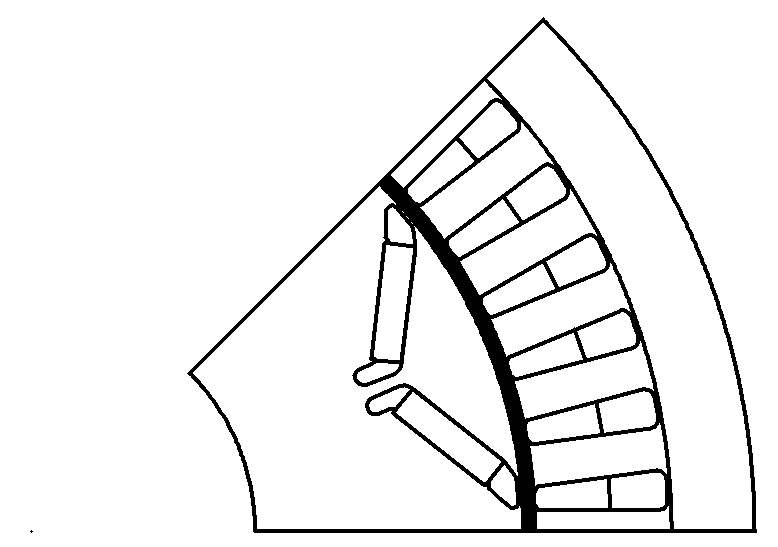
\includegraphics[width=0.47\linewidth]{dxf-orig} \hfill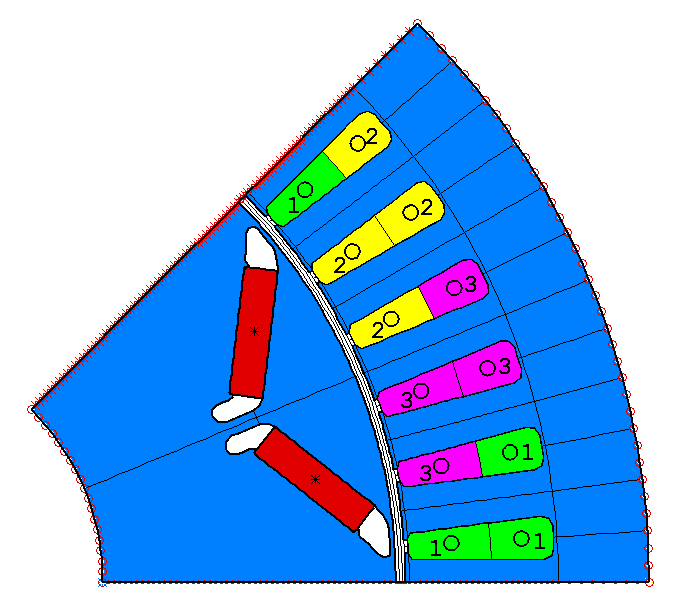
\includegraphics[width=0.4\linewidth]{femag-model}

The module meets the following requirements:
\begin{enumerate}
\item Identification of the airgap and the machine parts arranged inside and outside the airgap (stator, rotor)
 with their inside and outside diameters.
\item Identification of the symmetry axes with partitioning into the smallest possible area such that the complete
  machine model can be created by applying a sequence of reflection and copy/rotate functions.
\item Definition of the node densities of each area starting from the airgap to reach best results for
  cogging torque simulations.
\item Identification of the subregions winding, lamination and magnets for assigning their material properties.
\item Parametrized winding definition of distributed and concentrated one and two layer windings.
\end{enumerate}
The module is executable and cyn be invoked as follows:
\begin{verbatim}
python -m femagtools.dxfsl.conv [<options>] <DXF filename>
\end{verbatim}
%
\newpage
\enlargethispage{1cm}
\section{Processing steps}
\begin{enumerate}
\item
  Parse the DXF file with its lines, arcs and circles and create a NetworkX-Graph with nodes and edges.
\begin{center}
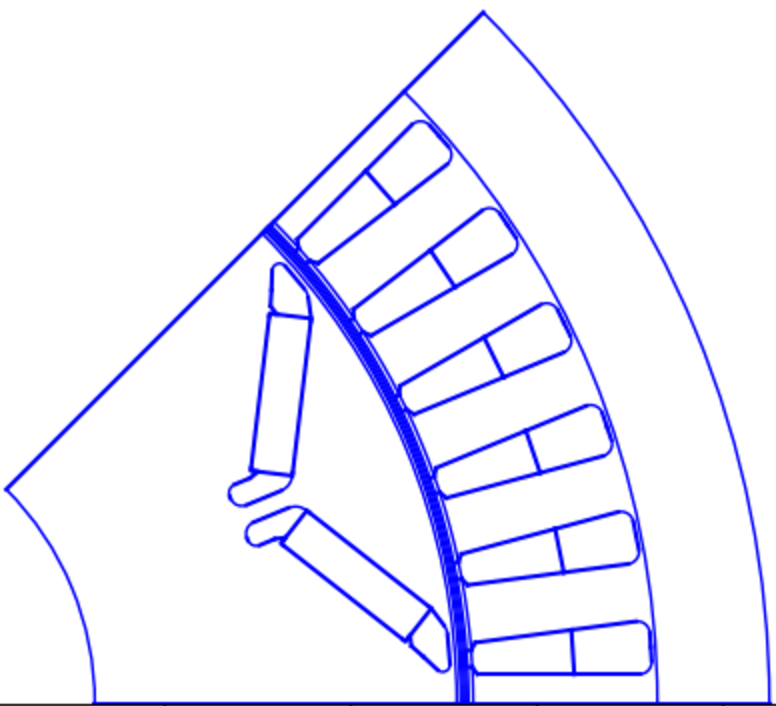
\includegraphics[width=0.45\linewidth]{step1}
\end{center}
\item Determine the graph cycles and identify the areas stator, rotor and airgap with their symmetry axes and extract
  the stator and rotor slots.

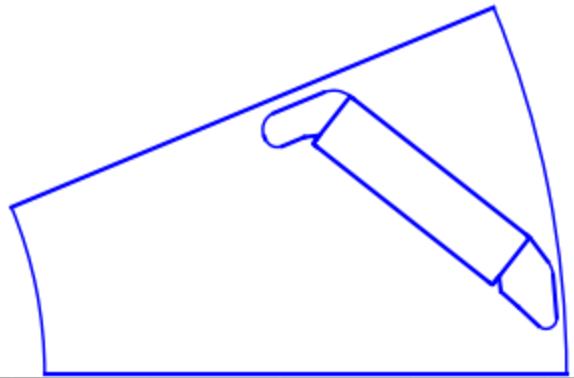
\includegraphics[width=0.45\linewidth]{step2}\hfill
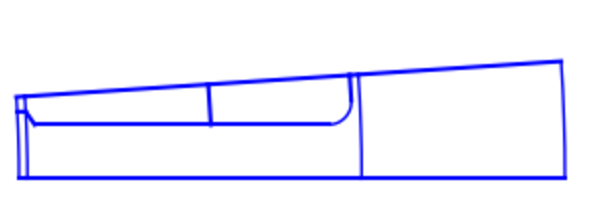
\includegraphics[width=0.45\linewidth]{step4}
\item
  Add auxiliary lines to simplify meshing.
\item
   output the model creation commands as FSL (Lua) script.
\end{enumerate}

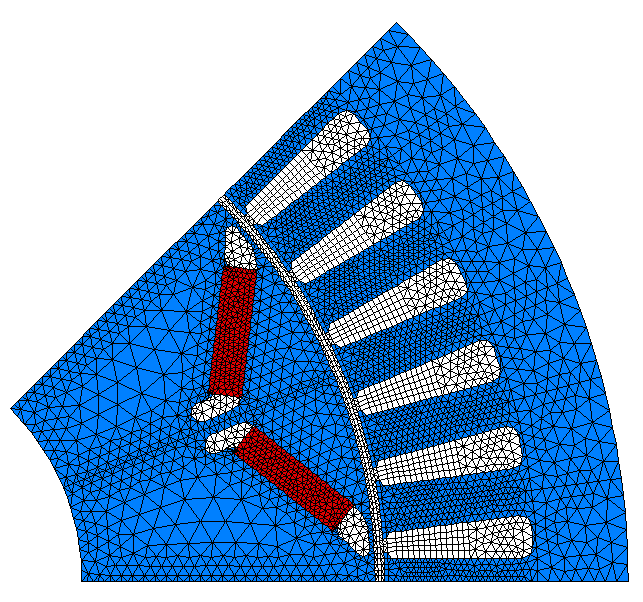
\includegraphics[width=0.45\linewidth]{mesh}\hfill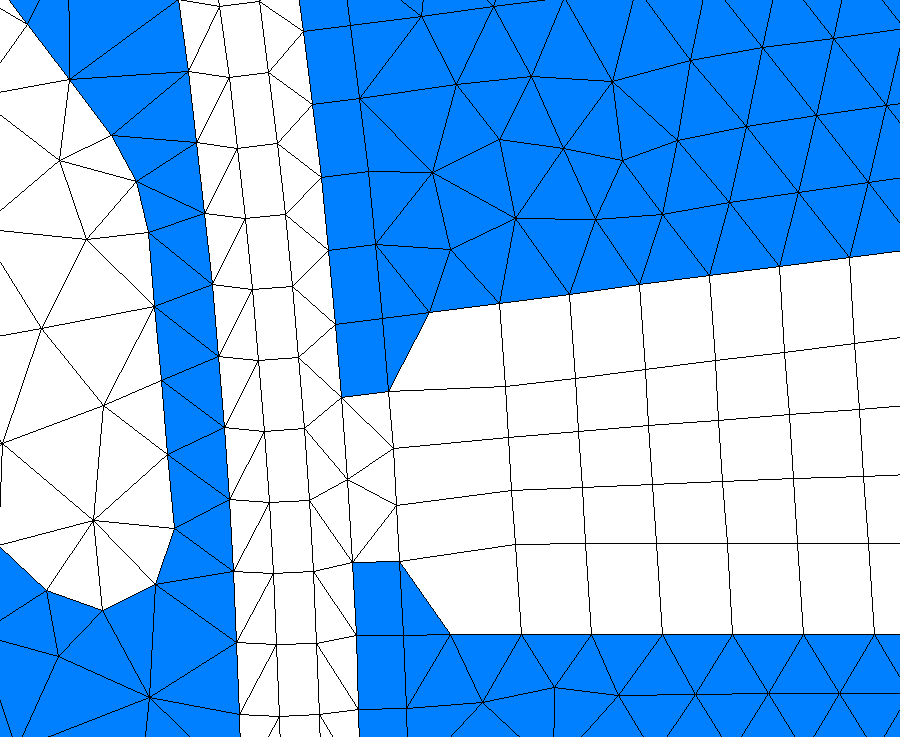
\includegraphics[width=0.45\linewidth]{airgap}
%
\section{Command line parameters}

The following
\begin{itemize}
\item filename of the source DXF
\item {\bfseries{\LongArg{fsl}}}\\
      create FSL script (default)

\item {\bfseries{\LongArg{split}}}\\
		check the geometry for intersecting lines and add intersection points.
       This option can be useful if no adequate symmetries and/or regions can be found.

\item {\bfseries{\LongArg{view}}}\\
		displays the geometry in a graphic. No further processing is done.

\item {\bfseries{\LongArg{plot}}}\\
		displays the results of different processing steps in a graphic.

%\item {\bfseries{\LongArg{airgap} Radius (float)}}\\
%		Wenn mehrere Luftspalt-Kandidaten vorhanden sind, wird die Verarbeitung abgebrochen und
%		die Kandidaten werden angezeigt. Mit diesem Parameter wird der innere Radius festgelegt.
%		Falls kein Luftspalt vorhanden ist, das Programm aber gleichwohl einen Luftspalt
%		identifiziert, kann die Luftspaltidentifikation mit einem negativen Wert unterbunden werden.

%\item {\bfseries{\LongArg{airgap2} Radius (float)}}\\
%		Wenn im Luftspalt zusätzliche, unnötige Linien vorhanden sind, können diese mit der
%		Angabe \Slanted{airgap2} eliminiert werden. Alle Linien zwischen \Slanted{airgap} und
%		\Slanted{airgap2} werden damit entfernt.

\item {\bfseries{\LongArg{rotor} in / out}}\\
		if a rotor only is included in the DXF file the type and position must be specificied.
		The value  {\bfseries in}
		or {\bfseries out} defines if the rotor is inside or outside the airgap.

\item {\bfseries{\LongArg{stator} in / out}}\\
		(see Argument \LongArg{rotor})

%\item {\bfseries{\LongArg{symtol} Toleranzwert (float)}}\\
%		Wenn ohne sichtbaren Grund keine Symmetrieachsen gefunden werden, können mit diesem Parameter
%		die Toleranzbedingungen beeinflussz werden.
%		(siehe auch \Slanted{rtol})

%\item {\bfseries{\LongArg{rtol} Relativer Toleranzwert (float)}}\\
%		Zum ermitteln, ob Knoten als \Slanted{gleich} zu betrachten sind, werden intern relative
%		und absolute Abweichungen toleriert. Der Default-Wert ist bei beiden 1e-03. Im Femag
%		entspricht dies der Variablen \Slanted{pickdist}.\\
%		Die Parameter \Slanted{rtol} und \Slanted{atol} sollten nur bei Maschinen übersteuert
%		werden, die mit dem CAD etwas ungenau konstruiert wurden.

%\item {\bfseries{\LongArg{atol} Absoluter Toleranzwert (float)}}\\
%		(siehe \Slanted{rtol})

%\item {\bfseries{\LongArg{debug}}}\\
%		Durch diese Option werden zusätzliche Informationen (z.B Plots) ausgegeben.
\end{itemize}

\section{Winding Area Detection}
The converter looks for closed areas in the geometry and tries to identify
the symmetry axes. The following image shows a stator with open slot areas:
\begin{center}
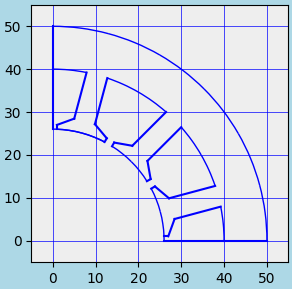
\includegraphics[width=0.45\linewidth]{BspStator}
\end{center}
In this example the converter is not able to identify the winding area.
The problem can be fixed by adding a connection line in the slot opening.

%Beispiel: Durch das Einziehen einer Verbindung im Nutschlitz
% wird die Wicklung und der am Luftspalt (airgap) liegende leere Bereich
%(Luft) erkannt und der Converter findet eine achsiale Symmetrieachse.
\begin{center}
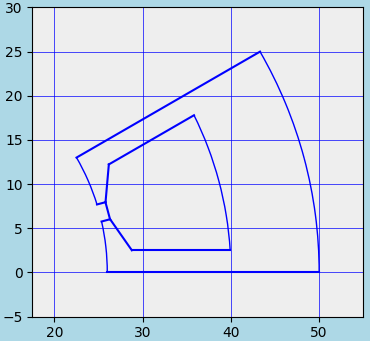
\includegraphics[width=0.45\linewidth]{BspWindings}
\end{center}
Note: the slot areas are normally left intact and are not divided horizontally or vertically.
If such a division is intended then separator lines must be included in the slot areas.
\end{document}
